\documentclass{beamer}

\usetheme{Antibes}

% Loading preambulo
% PREAMBULO ====================================================================

% Packages ---------------------------------------------------------------------

% Package to Portuguese language
\usepackage[brazilian]{babel}
% Packages to Figures
\usepackage{graphicx}
\usepackage{tikz}
% Packages to math symbols and expressions
\usepackage{amsfonts, amssymb, amsmath}
% Packages to insert code
\usepackage{listings} 
\usepackage{verbatim}
% Package to justify text
\usepackage[document]{ragged2e}
% Package to manage the bibliography
\usepackage[backend=biber, style=numeric, sorting=none]{biblatex}
% Package to facilitate quotations
\usepackage{csquotes}
% Package to use multicols
\usepackage{multicol}
% Packages for url
%	The package libertinus already loads hyperref
%\usepackage[colorlinks=true]{hyperref}
% Font
%   Fira
%\usepackage[sfdefault, lf]{FiraSans}
%   Libertinus
\usepackage{libertinus}
\renewcommand*\familydefault{\sfdefault} %% Only if the base font of the document is to be sans serif
% Colors
\usepackage{xcolor}
\usepackage{colortbl}
% Table
\usepackage{tabularray}
% Fill line
\usepackage{xhfill}

% Configurations ---------------------------------------------------------------

\AtBeginSection{
    \begin{frame}{\secname}
        \tableofcontents[currentsection,hideallsubsections]
    \end{frame}
}

\AtBeginSubsection{
    \begin{frame}{\subsecname}
        \tableofcontents[currentsection,subsectionstyle=show/shaded/hide, subsubsectionstyle=hide]
    \end{frame}
}

\AtBeginSubsubsection{
    \begin{frame}{\subsubsecname}
        \tableofcontents[currentsection,subsectionstyle=show/shaded/hide,subsubsectionstyle=show/shaded/hide/hide]
    \end{frame}
}

% Numbering slides
\setbeamertemplate{footline}[frame number]{}

% Getting rid of bottom navigation bars
\setbeamertemplate{navigation symbols}{}

% Margins
\setbeamersize{text margin left=20pt, text margin right=20pt}

% Colors
\definecolor{burgundy}{RGB}{133,24,42}
\definecolor{bloodred}{RGB}{147,5,5}

\setbeamercolor{structure}{fg=burgundy}

\setbeamercolor*{palette primary}{use=structure,fg=white,bg=structure.fg}
%\setbeamercolor*{palette secondary}{use=structure,fg=white,bg=structure.fg!75!black}
%\setbeamercolor*{palette tertiary}{use=structure,fg=white,bg=structure.fg!50!black}
\setbeamercolor*{palette quaternary}{fg=white,bg=bloodred}

%	hyperref
\hypersetup{
	colorlinks=true,
	urlcolor=blue,
	breaklinks=true}

% New commands -----------------------------------------------------------------

\NewTblrTableCommand \aula{\SetCell{bg=green!60,fg=white}}
\NewTblrTableCommand \prova{\SetCell{bg=red!80,fg=white}}
\NewTblrTableCommand \feriado{\SetCell{bg=blue!50,fg=white}}

\newcommand{\esta}[1]{\textbf{\underline{#1}}}

% Title
\title[GP 03]{Gerência de Projetos}
% Subtitle
\subtitle{Princípios do Gerenciamento de Projetos - Parte 2}
% Author of the presentation
\author[E.J.R. Silva]{Evandro J.R. Silva}
% date of the presentation
\date{}

\begin{document}
    
\begin{frame}
    \titlepage
\end{frame}

\begin{frame}{Sumário}
    \small
    \tableofcontents
\end{frame}

%===============================================================================
% SECTION 1 ====================================================================
%===============================================================================
\section{Princípios (Continuação)}

%-------------------------------------------------------------------------------
% SUBSECTION 1.1 ---------------------------------------------------------------
%-------------------------------------------------------------------------------
\subsection{Faça a adaptação de acordo com o contexto}

\begin{frame}{Faça a adaptação de acordo com o contexto}
	
\includegraphics[width=\textwidth]{imagens/figura01.png}
\end{frame}

\begin{frame}{Faça a adaptação de acordo com o contexto}
	\begin{itemize}
		\justifying
		\item Cada projeto é único. Portanto, a equipe do projeto deve utilizar uma abordagem ``suficiente'' para maximizar o valor, gerenciar custos e aumentar a velocidade ao elaborar a estratégia de desenvolvimento do projeto, levando em consideração o contexto, os objetivos, as partes interessadas, a governança e o ambiente do projeto. 
		\item A personalização de projetos pode aumentar a capacidade de criatividade, eficácia e produtividade de uma empresa, bem como sua capacidade de adaptação às mudanças nas condições do projeto.
	\end{itemize}
\end{frame}

\begin{frame}{Faça a adaptação de acordo com o contexto}
	\begin{itemize}
		\justifying
		\item Breve estudo de caso (\href{https://www.sciencedirect.com/science/article/pii/S1877050923004805?via\%3Dihub}{fonte})
		\begin{itemize}
			\justifying
			\item<1-> Em uma instituição pública, o \textit{tailoring} foi aplicado adaptando os processos, ferramentas e governança do PMBOK 7 ao contexto específico de restrições burocráticas, normas regulatórias e recursos limitados do setor público.
			\item<2-> Em vez de seguir uma metodologia rígida, a equipe customizou o ``just enough'' de processos para maximizar valor, reduzir custos e acelerar entregas, alinhando o desenvolvimento do projeto às particularidades organizacionais e ambientais.
			\item<3> \textbf{Resultado}: maior eficiência e alinhamento com os objetivos institucionais, evitando sobrecarga desnecessária de processos prescritivos.
		\end{itemize}
	\end{itemize}
\end{frame}

%-------------------------------------------------------------------------------
% SUBSECTION 1.2 ---------------------------------------------------------------
%-------------------------------------------------------------------------------
\subsection{Crie qualidade nos processos e nas entregas}

\begin{frame}{Crie qualidade nos processos e nas entregas}
	
\includegraphics[width=\textwidth]{imagens/figura02.png}
\end{frame}

\begin{frame}{Crie qualidade nos processos e nas entregas}
	\begin{itemize}
		\justifying
		\item Os gerentes de projeto devem continuar priorizando a qualidade para gerar entregas que atendam aos objetivos do projeto e estejam em conformidade com as necessidades, usos e padrões de aceitação especificados pelas partes interessadas relevantes.
		\item Garantir que os processos do projeto sejam aceitáveis e o mais eficazes possível faz parte da qualidade do projeto. A qualidade deve ser levada em consideração em todas as etapas do projeto. A equipe pode avaliar a qualidade das entregas por meio de auditorias e inspe-ções.
		\item Além disso, podem usar revisões e auditorias para confirmar o processo de garantia da qualidade.
	\end{itemize}
\end{frame}

\setbeamertemplate{background canvas}{
	\tikz[remember picture, overlay] \node[opacity=0.15,inner sep=0pt] at (current page.center){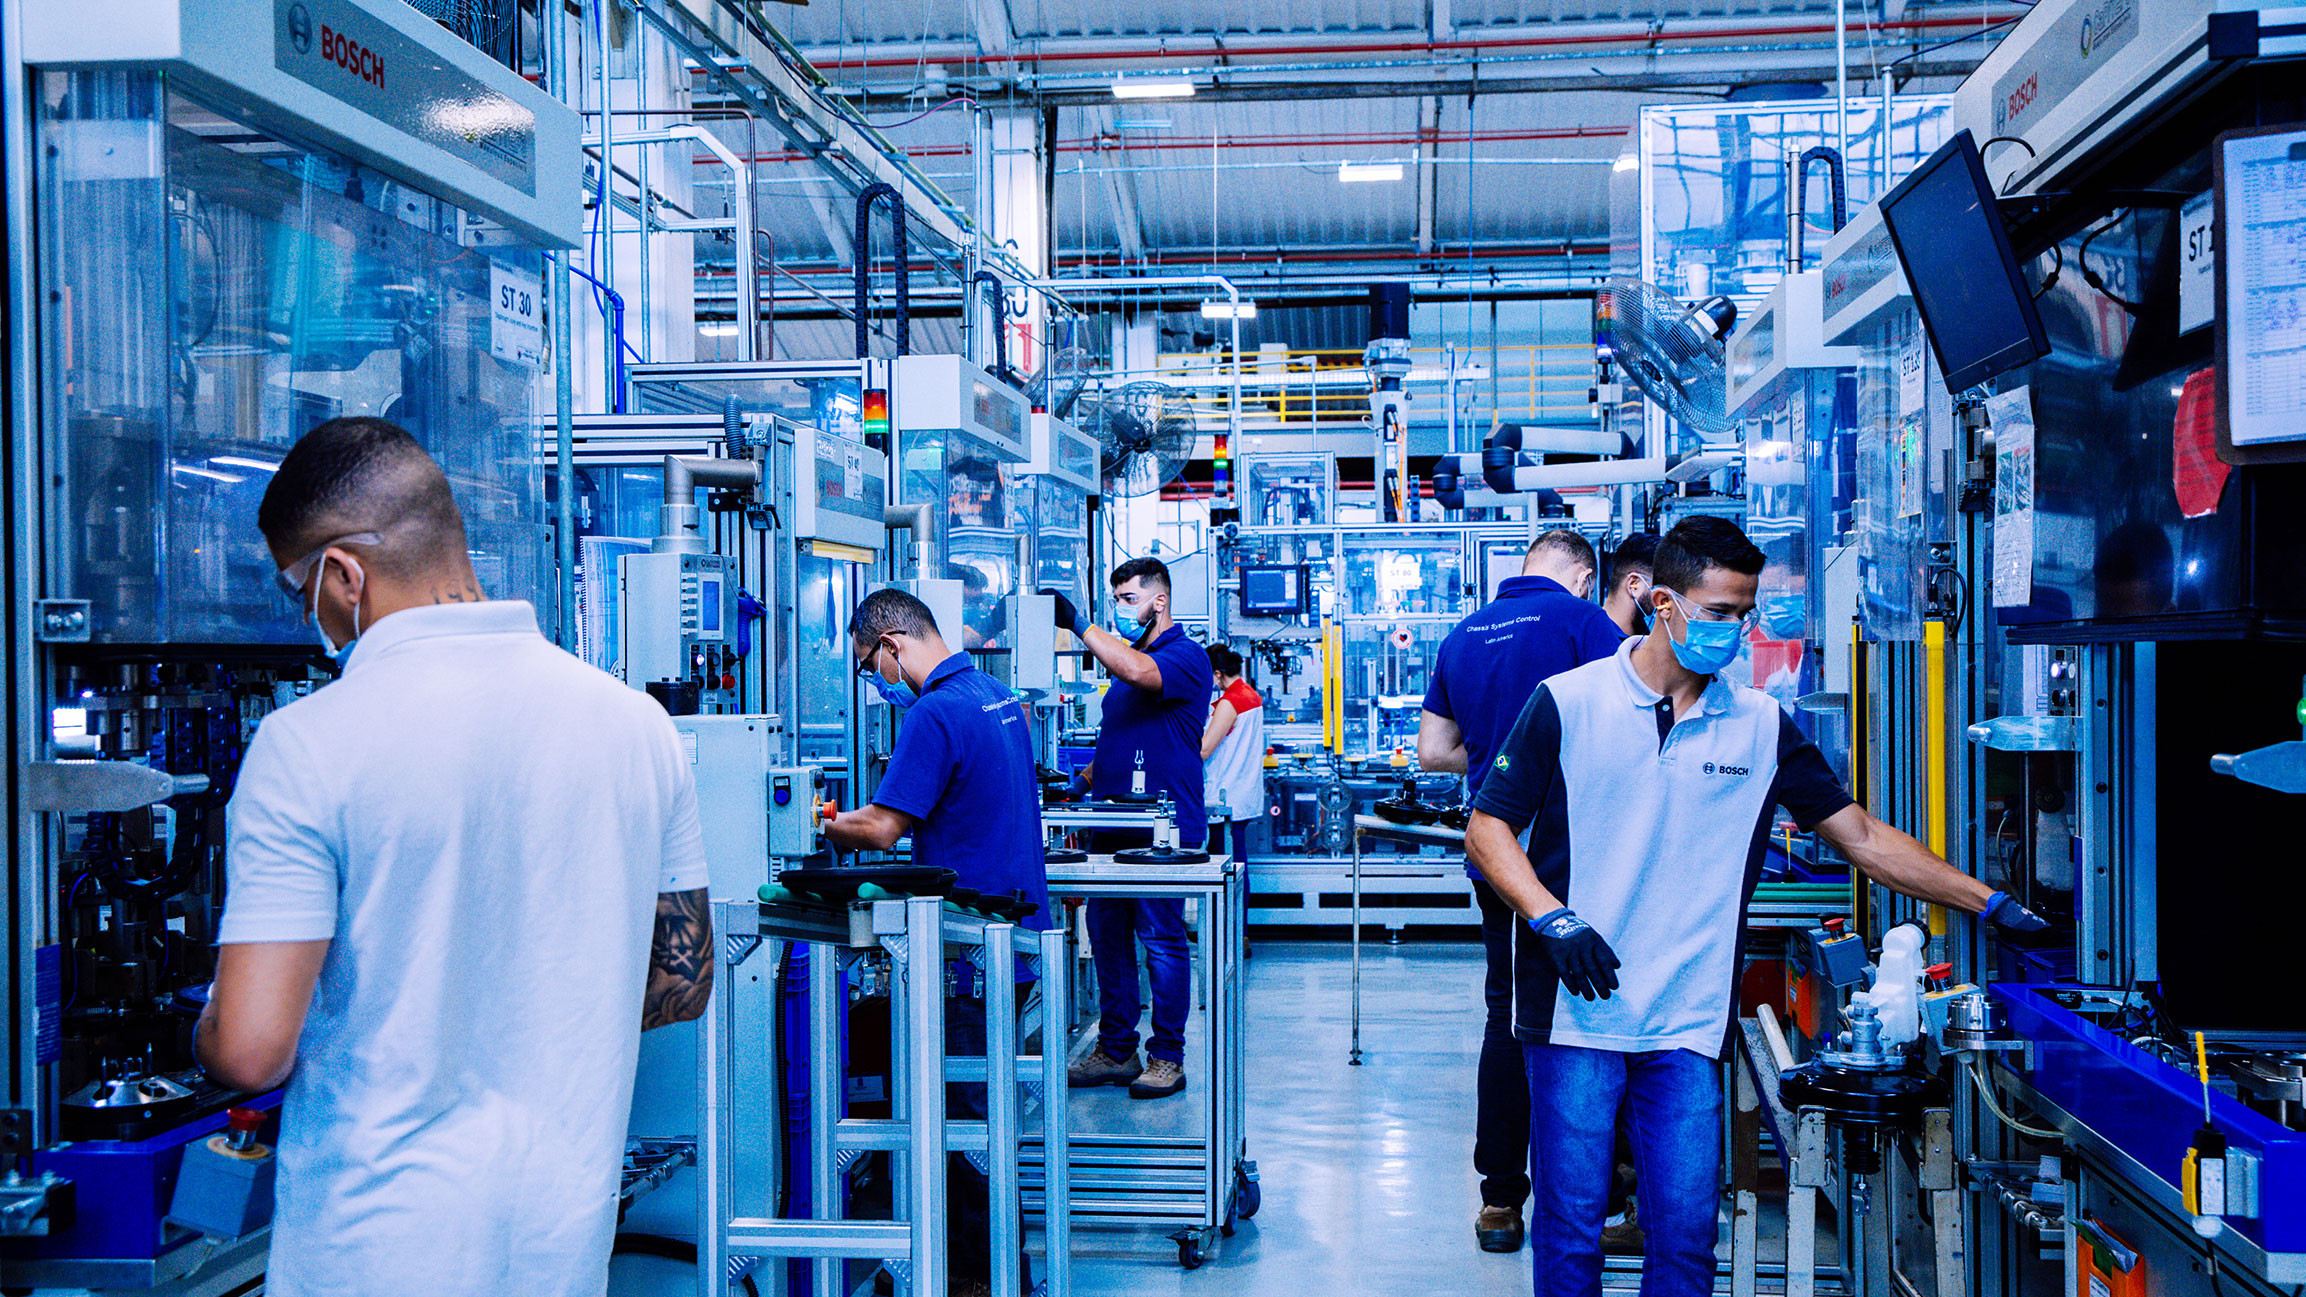
\includegraphics[width=\paperwidth,height=\paperheight]{imagens/celulas-de-manufatura.jpg}};}

\begin{frame}{Crie qualidade nos processos e nas entregas}
	\begin{itemize}
		\justifying
		\item Breve estudo de caso (\href{https://www.pmi.org/business-solutions/case-studies/using-a-pmi-disciplined-agile-approach-in-global-manufacturing}{fonte})
			\begin{itemize}
				\justifying
				\item<1-> Uma empresa global de manufatura adotou o  PMI Disciplined Agile $\circledR$ para integrar qualidade desde o início dos processos e entregas.
				\item<2-> Em vez de inspeções finais, a equipe incorporou práticas de qualidade contínua (\textit{quality built-in}) em todos os domínios, com foco em entregas que atendessem aos requisitos de \textit{stakeholders}, reduzindo defeitos e retrabalho. Isso incluiu ciclos iterativos de revisão e alinhamento com necessidades do cliente, elevando a qualidade dos produtos finais.
				\item<3-> \textbf{Resultado}: aumento significativo na velocidade de produção, produtividade da equipe e qualidade geral dos \textit{deliverables}.
			\end{itemize}
	\end{itemize}
\end{frame}

\setbeamertemplate{background canvas}[default]

%-------------------------------------------------------------------------------
% SUBSECTION 1.3 ---------------------------------------------------------------
%-------------------------------------------------------------------------------
\subsection{Navegue pela complexidade}

\begin{frame}{Navegue pela complexidade}
	
\includegraphics[width=\textwidth]{imagens/figura03.png}
\end{frame}

\begin{frame}{Navegue pela complexidade}
	\begin{itemize}
		\justifying
		\item A quantidade de riscos, ocorrências, circunstâncias e partes interessadas torna certos projetos mais complexos do que outros. 
		\item A complexidade é uma característica de um projeto que pode ser impactada pelo comportamento do sistema, pelo comportamento humano ou pela ambiguidade e imprevisibilidade do avanço tecnológico. 
		\item Portanto, a equipe do projeto deve ter habilidades de adaptação e estar aberta a adotar ideias inovadoras para lidar com a complexidade. Ela precisa reconhecer os componentes da complexidade e aplicar uma gama de técnicas para reduzir sua influência ou magnitude.
	\end{itemize}
\end{frame}

\setbeamertemplate{background canvas}{
	\tikz[remember picture, overlay] \node[opacity=0.15,inner sep=0pt] at (current page.center){\includegraphics[width=\paperwidth,height=\paperheight]{imagens/trem.jpg}};}
	
\begin{frame}{Navegue pela complexidade}
	\begin{itemize}
		\justifying
		\item Breve estudo de caso (\href{https://www.spoclearn.com/blog/project-management-complexity/}{fonte})
			\begin{itemize}
				\justifying
				\item<1-> Na modernização de um sistema ferroviário transnacional de mais de 3.000 km, a equipe enfrentou múltiplas jurisdições, desafios técnicos elevados e diversidade de \textit{stakeholders}.
				\item<2-> Aplicando pensamento holístico e planejamento iterativo do PMBOK 7 (com engajamento de stakeholders, análise de riscos e ajustes adaptativos), foram gerenciadas interdependências complexas, regulamen-tações variadas e incertezas ambientais.
				\item<3> \textbf{Resultado}: o projeto foi concluído dentro do orçamento e antes do prazo, com ganhos em eficiência operacional e satisfação dos clientes.
			\end{itemize}
	\end{itemize}
\end{frame}

\setbeamertemplate{background canvas}[default]

%-------------------------------------------------------------------------------
% SUBSECTION 1.4 ---------------------------------------------------------------
%-------------------------------------------------------------------------------
\subsection{Otimize as respostas ao risco}

\begin{frame}{Otimize as respostas ao risco}
	
\includegraphics[width=\textwidth]{imagens/figura04.png}
\end{frame}

\begin{frame}{Otimize as respostas ao risco}
	\begin{itemize}
		\justifying
		\item Todo projeto apresenta oportunidades e riscos, que podem ser positivos ou negativos. 
		\item Portanto, os gerentes de projeto devem abordar os riscos continuamente durante o projeto. Eles precisam avaliar a exposição ao risco, incluindo ameaças e oportunidades, para limitar os impactos adversos e maximizar os efeitos positivos nos resultados do projeto. Devem ser capazes de fornecer respostas adequadas à importância do risco, economicamente viáveis, aprovadas pelas partes interessadas relevantes e de responsabilidade de um indivíduo.
	\end{itemize}
\end{frame}

\setbeamertemplate{background canvas}{
	\tikz[remember picture, overlay] \node[opacity=0.15,inner sep=0pt] at (current page.center){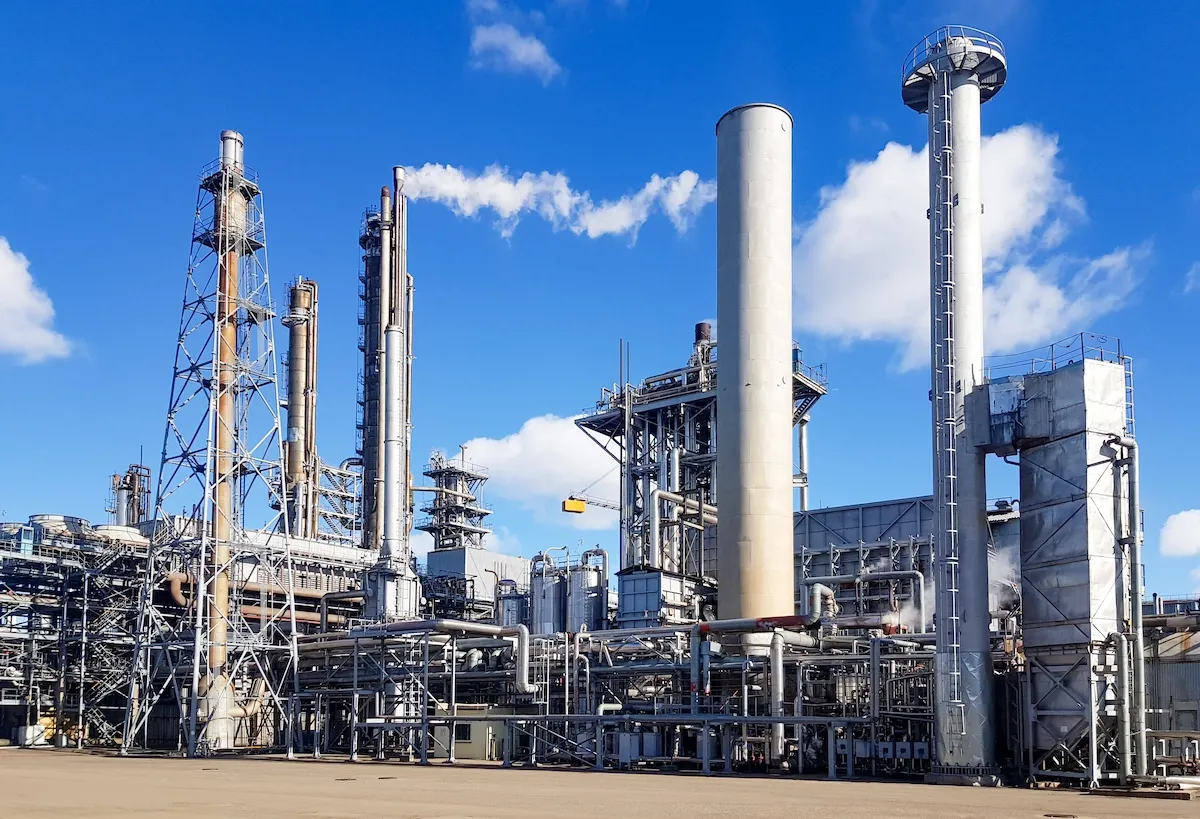
\includegraphics[width=\paperwidth,height=\paperheight]{imagens/refinery.png}};}
	
\begin{frame}{Otimize as respostas ao risco}
	\begin{itemize}
		\justifying
		\item Breve estudo de caso (\href{https://www.pmi.org/learning/library/risk-complex-projects-case-study-6308}{fonte})
		\begin{itemize}
			\justifying
			\item<1-> No projeto de construção de uma refinaria de petróleo em Jubail (Arábia Saudita), \textit{joint venture} entre Saudi Aramco e TOTAL (orçamento de US\$ 12 bilhões), a equipe atuou como ``Program Risk Engineer'' em um ambiente de alta complexidade (índice Nelson 10.6, 15 pacotes de contratação, recessão global).
			\item<2-> Usando matriz 5x5 de probabilidade/impacto, identificação iterativa e respostas otimizadas (ex.: retender pacotes para economizar até US\$ 500 milhões, introdução de contratante principal para reduzir coordenação), foram maximizados riscos positivos (economia) e minimizados negativos (atrasos e sobrecusto).
			\item<3> \textbf{Resultado}: a abordagem equilibrou custo, cronograma e conformidade local.
		\end{itemize}
	\end{itemize}
\end{frame}

\setbeamertemplate{background canvas}[default]

%-------------------------------------------------------------------------------
% SUBSECTION 1.5 ---------------------------------------------------------------
%-------------------------------------------------------------------------------
\subsection{Adote a capacidade de adaptação e resiliência}

\begin{frame}{Adote a capacidade de adaptação e resiliência}
	
\includegraphics[width=\textwidth]{imagens/figura05.png}
\end{frame}

\begin{frame}{Adote a capacidade de adaptação e resiliência}
	\begin{itemize}
		\justifying
		\item Os gerentes de projeto devem ser capazes de se adaptar e responder às mudanças se quiserem aprimorar seus projetos. 
		\item Portanto, a equipe do projeto deve incluir adaptação e resiliência em seus métodos para facilitar a mudança, superar desafios e alcançar os objetivos do projeto. 
		\item Isso deve abranger tanto mudanças externas quanto internas. Assim, os gerentes de projeto e suas equipes devem aprender a se ajustar às novas mudanças.
	\end{itemize}
\end{frame}

\setbeamertemplate{background canvas}{
	\tikz[remember picture, overlay] \node[opacity=0.15,inner sep=0pt] at (current page.center){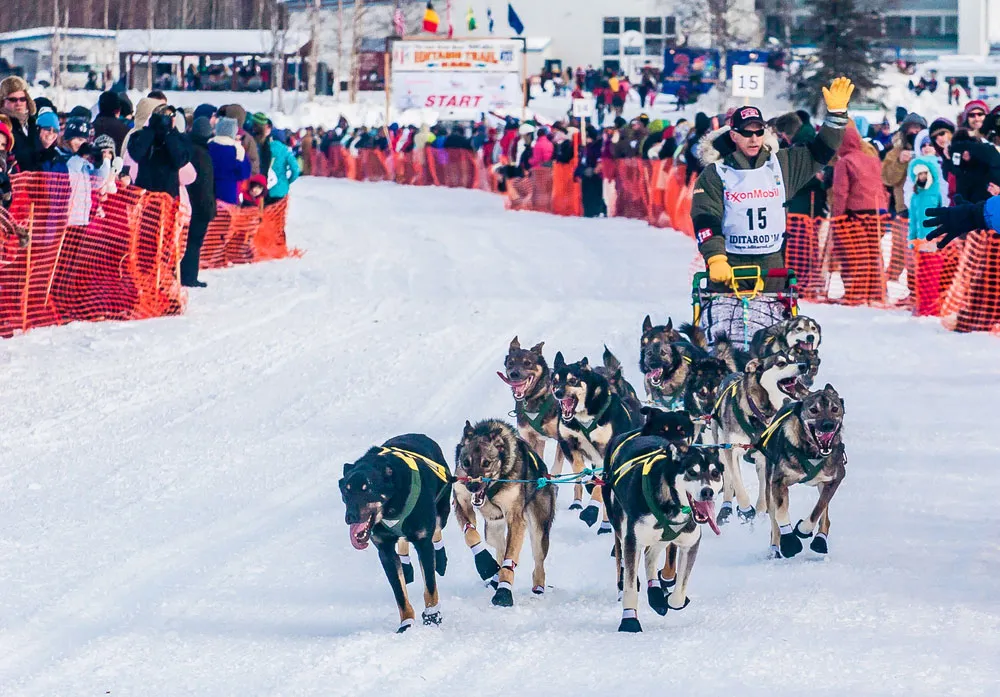
\includegraphics[width=\paperwidth,height=\paperheight]{imagens/iditarod.png}};}

\begin{frame}{Adote a capacidade de adaptação e resiliência}
	\begin{itemize}
		\justifying
		\item Breve estudo de caso (\href{https://blog.iil.com/applying-pmbok-guide-7th-edition-to-projects/}{fonte})
		\begin{itemize}
			\justifying
			\item<1-> Durante a corrida Iditarod (Alasca, março 2020), um evento de 1.000 milhas em meio ao início da pandemia de COVID-19, a organização enfrentou recusas de vilarejos em checkpoints, cancelamento de eventos e isolamento dos competidores.
			\item<2-> Aplicando o princípio de resiliência, foram mantidos planos A/B/C, decisões adiadas até o último momento, colaboração com \textit{stakeholders} diversos (veterinários, anciãos, voluntários) e aprendizado contínuo entre checkpoints.
			\item<3> \textbf{Resultado}: a corrida foi concluída com todos os competidores e cães em segurança; lições geraram mudanças permanentes (ex.: roteiros alternativos em 2021).
		\end{itemize}
	\end{itemize}
\end{frame}

\setbeamertemplate{background canvas}[default]

%-------------------------------------------------------------------------------
% SUBSECTION 1.6 ---------------------------------------------------------------
%-------------------------------------------------------------------------------
\subsection{Aceite a mudança para alcançar o futuro estado previsto}

\begin{frame}{Aceite a mudança para alcançar o futuro estado previsto}
	
\includegraphics[width=\textwidth]{imagens/figura06.png}
\end{frame}

\begin{frame}{Aceite a mudança para alcançar o futuro estado previsto}
	\begin{itemize}
		\justifying
		\item Existem duas possíveis fontes de mudança em um projeto: internas e externas. Pode ser difícil permitir mudanças em um projeto, pois isso exige certa flexibilidade e conhecimento das pessoas, tanto dentro quanto fora da equipe. 
		\item O gerente de projeto é responsável por garantir que as estratégias corretas de gestão de mudanças sejam aplicadas. Ele deve incluir as partes interessadas e incentivá-las a abraçar a mudança para garantir o sucesso.
	\end{itemize}
\end{frame}

\setbeamertemplate{background canvas}{
	\tikz[remember picture, overlay] \node[opacity=0.15,inner sep=0pt] at (current page.center){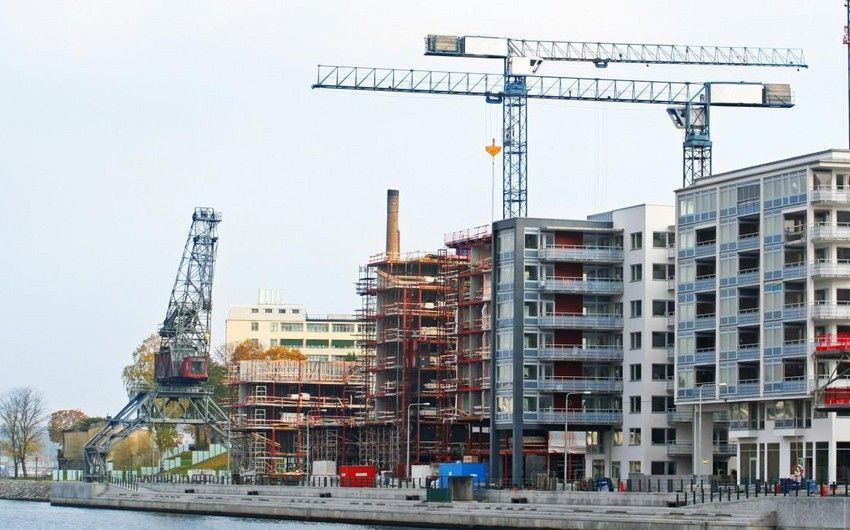
\includegraphics[width=\paperwidth,height=\paperheight]{imagens/construction.jpg}};}

\begin{frame}{Aceite a mudança para alcançar o futuro estado previsto}
	\begin{itemize}
		\justifying
		\item Breve estudo de caso (\href{https://www.pmi.org/learning/library/project-based-organizations-change-management-6471}{fonte})
		\begin{itemize}
			\justifying
			\item<1-> Na \textit{Construction Sweden} (empresa sueca de construção baseada em projetos), foi implementada a ferramenta \textit{Visual Planning} (VP), inspirada na Toyota, para transformar o planejamento tradicional em visual e colaborativo (post-its em paredes, envolvimento de subcontratados).
			\item<2-> Apesar de desafios típicos de organizações projetizadas (descentrali-zação, resistência cultural e comunicação insuficiente), a mudança foi ancorada com coalizões guias, educação e benefícios operacionais por projeto.
			\item<3> \textbf{Resultado}: maior compromisso das equipes, redução de tempo de produção e maior alinhamento com o futuro estado de eficiência e colaboração desejado.
		\end{itemize}
	\end{itemize}
\end{frame}

\setbeamertemplate{background canvas}[default]


%===============================================================================
% SECTION 2 ====================================================================
%===============================================================================
\section{Atividade}

\begin{frame}{Atividade}
    \begin{itemize}
        \justifying
        \item Vamos nos dividir novamente em grupos.
        \item Cada grupo deverá analisar os problemas disponíveis nos próximos slides e, para cada problema:
        \begin{itemize}
        	\justifying
        	\item Identificar qual princípio está sendo negligenciado.
        	\item Identificar/sumarizar o problema central.
        	\item Propor ações corretivas.
        	\item Identificar riscos financeiros, reputacionais e humanos.
        	\item Avaliar consequências das decisões.
        \end{itemize}
        \item Os grupos terão um tempo para discutir sobre cada problema e, ao fim, vamos debater sobre as respostas.
    \end{itemize}
\end{frame}

%-------------------------------------------------------------------------------
% SUBSECTION 2.1 ---------------------------------------------------------------
%-------------------------------------------------------------------------------
\subsection{Problema 1 - Implantação de Sistema de Gestão em Hospital Regional}

\begin{frame}{Problema 1 - Implantação de Sistema de Gestão em Hospital Regional}
	\begin{itemize}
		\justifying
		\item Um hospital regional público decidiu implantar um sistema integrado de gestão hospitalar que inclui:
			\begin{itemize}
				\justifying
				\item Prontuário eletrônico.
				\item Controle de leitos.
				\item Agendamento de exames.
				\item Integração com farmácia hospitalar.
			\end{itemize}
		\item A empresa contratada possui uma \textbf{metodologia padrão baseada em práticas tradicionais de gerenciamento de projetos}, com forte documentação, ciclos de aprovação e fases sequenciais.
	\end{itemize}
\end{frame}

\begin{frame}{Problema 1 - Implantação de Sistema de Gestão em Hospital Regional}
	\begin{itemize}
		\justifying
		\item Durante o início do projeto, surgem alguns desafios:
			\begin{itemize}
				\justifying
				\item A rotina hospitalar é altamente dinâmica.
				\item Médicos e enfermeiros têm pouco tempo para participar de reuniões longas.
				\item Mudanças emergenciais são frequentes.
				\item O hospital precisa de funcionalidades prioritárias funcionando rapidamente.
			\end{itemize}
		\item Mesmo assim, a empresa insiste em seguir rigorosamente sua metodologia padrão, sem adaptações.
		\item Após três meses:
			\begin{itemize}
				\item Apenas documentos foram produzidos.
				\item Nenhuma funcionalidade foi implementada.
				\item A direção do hospital demonstra frustração.
			\end{itemize}
	\end{itemize}
\end{frame}

\begin{frame}{Problema 1 - Implantação de Sistema de Gestão em Hospital Regional}
	\begin{itemize}
		\justifying
		\small
		\item \textbf{Dilema}: seguir rigidamente a metodologia corporativa ou adaptar o gerenciamento do projeto ao contexto do hospital.
		\item Perguntas norteadoras
			\begin{itemize}
				\justifying
				\footnotesize
				\item \textbf{Compreensão}
					\begin{itemize}
						\justifying
						\scriptsize
						\item Quais características do ambiente hospitalar tornam esse projeto diferente de outros projetos de software?
						\item Por que uma metodologia padrão pode não funcionar bem em todos os contextos?
					\end{itemize}
				\item \textbf{Análise}
					\begin{itemize}
						\justifying
						\scriptsize
						\item Quais problemas podem surgir quando práticas de gerenciamento não são adaptadas ao ambiente do projeto?
						\item Que elementos da metodologia poderiam ser ajustados sem comprometer o controle do projeto?
					\end{itemize}
				\item \textbf{Tomada de decisão}
					\begin{itemize}
						\justifying
						\scriptsize
						\item Que adaptações poderiam ser feitas na abordagem de gerenciamento desse projeto?
						\item Como equilibrar padronização organizacional e flexibilidade no gerenciamento de projetos?
					\end{itemize}
			\end{itemize}
	\end{itemize}
\end{frame}

%-------------------------------------------------------------------------------
% SUBSECTION 2.2 ---------------------------------------------------------------
%-------------------------------------------------------------------------------
\subsection{Problema 2 - Desenvolvimento de Sistema para Controle de Medicamentos}

\begin{frame}{Problema 2 - Desenvolvimento de Sistema para Controle de Medicamentos}
	\begin{itemize}
		\justifying
		\item Uma empresa de tecnologia foi contratada para desenvolver um sistema de controle de medicamentos para redes de farmácias. O sistema deverá:
			\begin{itemize}
				\justifying
				\item Registrar entradas e saídas de medicamentos.
				\item Controlar validade dos produtos.
				\item Gerar alertas para recolhimento de lotes.
			\end{itemize}
		\item Devido à forte concorrência no mercado, a empresa decide acelerar o desenvolvimento. Para cumprir o prazo:
			\begin{itemize}
				\justifying
				\item Testes são reduzidos.
				\item Revisões de código são simplificadas.
				\item Documentação é considerada opcional.
			\end{itemize}
		\item O sistema é entregue dentro do prazo. No entanto, após a implantação:
			\begin{itemize}
				\justifying
				\item Alguns medicamentos aparecem duplicados no sistema.
				\item Alertas de validade não funcionam corretamente.
				\item Farmácias enfrentam problemas regulatórios.
			\end{itemize}
	\end{itemize}
\end{frame}

\begin{frame}{Problema 2 - Desenvolvimento de Sistema para Controle de Medicamentos}
	\begin{itemize}
		\justifying
		\item \textbf{Dilema}: velocidade de entrega versus garantia de qualidade.
		\item Perguntas norteadoras
			\begin{itemize}
				\item \textbf{Compreensão}
					\begin{itemize}
						\justifying
						\item Qual é o objetivo principal do sistema desenvolvido para as farmácias?
						\item Por que a qualidade é especialmente importante em sistemas que lidam com medicamentos?
					\end{itemize}
				\item \textbf{Análise}
					\begin{itemize}
						\justifying
						\item Como decisões tomadas durante o processo de desenvolvimento afetaram a qualidade do produto?
						\item Que práticas poderiam ter sido implementadas para garantir qualidade sem comprometer totalmente o prazo?
					\end{itemize}
				\item \textbf{Tomada de decisão}
					\begin{itemize}
						\justifying
						\item Que tipos de processos ajudam a garantir qualidade em projetos de software?
						\item Como equilibrar velocidade de entrega e confiabilidade do sistema?
					\end{itemize}
			\end{itemize}
	\end{itemize}
\end{frame}

%-------------------------------------------------------------------------------
% SUBSECTION 2.3 ---------------------------------------------------------------
%-------------------------------------------------------------------------------
\subsection{Problema 3 - Implantação de Sistema Nacional de Identidade Digital}

\begin{frame}{Problema 3 - Implantação de Sistema Nacional de Identidade Digital}
	\begin{itemize}
		\justifying
		\item O Governo Federal iniciou um projeto para criar um sistema nacional de identidade digital. O sistema precisa integrar:
			\begin{itemize}
				\item Bases de dados estaduais.
				\item Sistemas da Polícia Federal.
				\item Registros civis.
				\item Plataformas bancárias.
				\item Serviços digitais do governo.
			\end{itemize}
		\item Além disso:
			\begin{itemize}
				\justifying
				\item Cada Estado possui infraestrutura tecnológica diferente.
				\item Há diferentes legislações estaduais.
				\item Múltiplas empresas participam do projeto.
				\item Milhões de cidadãos serão impactados.
			\end{itemize}
		\item Durante a execução, surgem dificuldades de integração entre sistemas. Alguns estados atrasam a entrega de dados e outros utilizam formatos incompatíveis.
	\end{itemize}
\end{frame}

\begin{frame}{Problema 3 - Implantação de Sistema Nacional de Identidade Digital}
	\begin{itemize}
		\justifying
		\item \textbf{Dilema}: gerenciar um projeto altamente interdependente com múltiplos atores e sistemas.
		\item Perguntas norteadoras
			\begin{itemize}
				\item \textbf{Compreensão}
					\begin{itemize}
						\justifying
						\item Quais fatores tornam esse projeto particularmente complexo?
						\item Por que projetos governamentais de grande escala tendem a apresentar alta complexidade?
					\end{itemize}
				\item \textbf{Análise}
					\begin{itemize}
						\justifying
						\item Como a interdependência entre sistemas pode gerar dificuldades na execução do projeto?
						\item De que forma a falta de coordenação entre instituições pode aumentar a complexidade do projeto?
					\end{itemize}
				\item \textbf{Tomada de decisão}
					\begin{itemize}
						\justifying
						\item Que estratégias poderiam ajudar a lidar com a complexidade desse projeto?
						\item Que tipo de estrutura de governança poderia facilitar a coordenação entre diferentes instituições?
					\end{itemize}
			\end{itemize}
	\end{itemize}
\end{frame}

%-------------------------------------------------------------------------------
% SUBSECTION 2.4 ---------------------------------------------------------------
%-------------------------------------------------------------------------------
\subsection{Problema 4 - Construção de Parque Eólico em Região Costeira}

\begin{frame}{Problema 4 - Construção de Parque Eólico em Região Costeira}
	\begin{itemize}
		\justifying
		\item Uma empresa de energia iniciou um projeto para construir um parque eólico em uma região costeira. O projeto envolve:
			\begin{itemize}
				\justifying
				\item Aquisição de turbinas importadas.
				\item Construção de fundações marítimas.
				\item Conexão com rede elétrica nacional.
			\end{itemize}
		\item Durante o planejamento foram identificados alguns riscos:
			\begin{itemize}
				\justifying
				\item Atrasos no transporte internacional das turbinas.
				\item Condições climáticas adversas.
				\item Mudanças na regulamentação ambiental.
			\end{itemize}
		\item Apesar disso, a direção da empresa decide não investir muito em planejamento de riscos, para reduzir custos iniciais. Meses depois:
			\begin{itemize}
				\justifying
				\item Uma tempestade forte danifica parte das estruturas.
				\item Entrega de turbinas é atrasada.
				\item Custos aumentam significativamente.
			\end{itemize}
	\end{itemize}
\end{frame}

\begin{frame}{Problema 4 - Construção de Parque Eólico em Região Costeira}
	\begin{itemize}
		\justifying
		\item \textbf{Dilema}: investir em gestão preventiva de riscos ou reagir apenas quando os problemas ocorrem.
		\item Perguntas norteadoras
			\begin{itemize}
				\item \textbf{Compreensão}
					\begin{itemize}
						\justifying
						\item Quais são os principais riscos associados ao projeto de construção do parque eólico?
						\item Por que projetos de infraestrutura costumam apresentar riscos elevados?
					\end{itemize}
				\item \textbf{Análise}
					\begin{itemize}
						\justifying
						\item Como a falta de planejamento de riscos contribuiu para os problemas enfrentados pelo projeto?
						\item Que estratégias poderiam ter reduzido os impactos desses riscos?
					\end{itemize}
				\item \textbf{Tomada de decisão}
					\begin{itemize}
						\justifying
						\item Que ferramentas podem ser utilizadas para identificar e analisar riscos em projetos?
						\item Como decidir quando vale a pena investir em medidas preventivas?
					\end{itemize}
			\end{itemize}
	\end{itemize}
\end{frame}

%-------------------------------------------------------------------------------
% SUBSECTION 2.5 ---------------------------------------------------------------
%-------------------------------------------------------------------------------
\subsection{Problema 5 - Projeto de Plataforma de Ensino Durante Crise Sanitária}

\begin{frame}{Problema 5 - Projeto de Plataforma de Ensino Durante Crise Sanitária}
	\begin{itemize}
		\justifying
		\item Uma universidade iniciou um projeto para desenvolver uma nova plataforma de ensino digital. Inicialmente, o projeto tinha cronograma de \textbf{18 meses}. Durante o desenvolvimento ocorre uma crise sanitária que obriga a universidade a suspender aulas presenciais. Subitamente:
			\begin{itemize}
				\justifying
				\item Milhares de alunos precisam estudar remotamente.
				\item Professores não estão preparados para ensino online.
				\item A plataforma ainda não está pronta.
			\end{itemize}
		\item A universidade decide antecipar o lançamento da plataforma em poucos meses. A equipe do projeto precisa:
			\begin{itemize}
				\justifying
				\item Reorganizar prioridades.
				\item Trabalhar com recursos limitados.
				\item Adaptar rapidamente funcionalidades.
			\end{itemize}
	\end{itemize}
\end{frame}

\begin{frame}{Problema 5 - Projeto de Plataforma de Ensino Durante Crise Sanitária}
	\begin{itemize}
		\item \textbf{Dilema}: responder rapidamente a uma crise sem comprometer totalmente o projeto.
		\item Perguntas norteadoras
			\begin{itemize}
				\item \textbf{Compreensão}
				\begin{itemize}
					\justifying
					\item Que mudança inesperada ocorreu durante o projeto?
					\item Por que a crise sanitária exigiu adaptação imediata do projeto?
				\end{itemize}
				\item \textbf{Análise}
				\begin{itemize}
					\justifying
					\item Como a equipe do projeto pode demonstrar resiliência diante dessa situação?
					\item Quais riscos surgem quando um projeto precisa acelerar drasticamente sua entrega?
				\end{itemize}
				\item \textbf{Tomada de decisão}
				\begin{itemize}
					\justifying
					\item Que estratégias podem ajudar equipes de projeto a se adaptar a mudanças inesperadas?
					\item Como manter o desempenho da equipe em situações de grande pressão?
				\end{itemize}
			\end{itemize}
	\end{itemize}
\end{frame}

%-------------------------------------------------------------------------------
% SUBSECTION 2.6 ---------------------------------------------------------------
%-------------------------------------------------------------------------------
\subsection{Problema 6 - Transformação Digital de Banco Tradicional}

\begin{frame}{Problema 6 - Transformação Digital de Banco Tradicional}
	\begin{itemize}
		\justifying
		\item Um banco tradicional iniciou um grande programa de transformação digital para competir com fintechs. O projeto envolve:
			\begin{itemize}
				\justifying
				\item Desenvolvimento de aplicativos móveis.
				\item Automação de processos internos.
				\item Substituição de sistemas legados.
				\item Criação de novos serviços digitais.
			\end{itemize}
		\item Entretanto, muitos gerentes da organização resistem às mudanças. Alguns departamentos:
			\begin{itemize}
				\justifying
				\item Continuam utilizando processos antigos.
				\item Evitam adotar novas ferramentas.
				\item Demonstram receio de perder funções ou influência.
			\end{itemize}
		\item O projeto avança tecnicamente, mas a adoção das novas soluções é baixa.
	\end{itemize}
\end{frame}

\begin{frame}{Problema 6 - Transformação Digital de Banco Tradicional}
	\begin{itemize}
		\justifying
		\item \textbf{Dilema}: implementar tecnologia nova em uma organização resistente à mudança.
		\item Perguntas norteadoras
		\begin{itemize}
			\item \textbf{Compreensão}
			\begin{itemize}
				\justifying
				\item Qual é o objetivo da transformação digital do banco?
				\item Por que mudanças organizacionais costumam gerar resistência?
			\end{itemize}
			\item \textbf{Análise}
			\begin{itemize}
				\justifying
				\item Como a resistência dos funcionários pode comprometer o sucesso do projeto?
				\item Quais fatores culturais influenciam a aceitação de mudanças em organizações tradicionais?
			\end{itemize}
			\item \textbf{Tomada de decisão}
			\begin{itemize}
				\justifying
				\item Que estratégias podem ajudar a reduzir a resistência à mudança?
				\item Como envolver colaboradores no processo de transformação organizacional?
			\end{itemize}
		\end{itemize}
	\end{itemize}
\end{frame}

%===============================================================================
% FIM ==========================================================================
%===============================================================================
\section{Fim}

\begin{frame}
    \centering
    \Large
    FIM
\end{frame}
    
\end{document}
